\chapter{Evaluation}
\section{Meeting Investigators from Industry} 
In order to gain feedback from the target end-users of this tool, we arranged a meeting with Mat Stanley, a Detective Sergeant of a London Metropolitan Police cryptocurrency investigation unit and, in order to also gain a private sector industry perspective, Iggy Azad who is a senior investigator at Coinbase.
\\\\
I arranged the meeting with the goal of obtaining qualitative feedback on \textit{Radar} based on their domain knowledge and experiences investigating cryptocurrency crime and learn how they currently achieve this using existing tools. We used this opportunity to find out more about the offerings of the proprietary software on the market that they have had experience with, such as ChainAnalysis, in order to compare the strengths and shortcomings of existing proprietary solutions.

\subsection{Successes and Weaknesses}
From the meeting with Mat and Iggy, where we demonstrated the current functionality of the tool, we obtained qualitative feedback such that we were able to identify areas of success and areas of weakness in the current implementation. These areas are summarised below:

\begin{itemize}
    \item \textbf{Weakness}: The different types of nodes aren't very clear (\textit{Implicit: We had to explain what the different types of nodes represent}).
    \item \textbf{Success}: The date and price filtering functionality is often very valuable to investigators. This is often particularly useful when tracing funds through a mixing service [see mixing services in background section \ref{background-mixing-service}]. 
    \item \textbf{Success}: Displaying the historical exchange rate is also very important to investigators; this enables them to better understand the true value of the flow of funds, which may be otherwise difficult without historical exchange rates due to the volatility in the value of Bitcoin. 
    \item \textbf{Success \& Weakness}: The Path Finding feature is very useful in investigations, yet not a feature provided by some of the software products they currently use. However, It would be useful to be able to type the name of a wallet rather than a specific address and the path finding functionality to be extended to support paths between any two wallets or any wallet and specific address.
    \item \textbf{Success}: Clustering using the wallet information obtained in section \ref{section-entity-tagging} will prove extremely useful; this data is also provided by their ChainAnalysis software. 
    \item \textbf{Success}: The ability to toggle on/off clustering heuristics is very desirable and not provided by several other solutions. 
    \item \textbf{Success \& Weakness}: Very common usage is to add additional information to compliment an investigation, so being able to do so through the custom node feature is very useful; however, adding information such as Photographic ID is not usually required at this stage of the investigation. The tool will be used in the run-up to issuing a warrant to obtain identification from exchanges (who should have it due to KYC [see Know Your Customer in background section \ref{background-kyc}). Additionally, it would be more intuitive to store this data with a particular node, rather than existing as a separate node itself. 
    \item \textbf{Weakness}: Secure data storage not addressed by current deployment: If storing investigation specific data, a secure solution is needed such that only the user could access it. 
\end{itemize}

\subsection{Desirable features}
Further to our conversation with Mat and Iggy, we were able to curate a list of features that would be useful to someone wishing to investigate cryptocurrency using \textit{Radar}. These features are:
\begin{itemize}
    \item Support for several cryptocurrencies. Namely: Ethereum, Litecoin, Bitcoin, Bitcoin Cash, Dash
    \item Ability to save a graph state as an investigation and come back to it later
    \item Ability to export the data from an investigation, often in CSV format to provide evidence for cases - needs to be digestible by a jury.
    \item Ability to set up notifications/watches for state changes on entities - e.g an address/wallet receives or spends funds 
    \item Automatically detect and alert when an address re-surfaces in a new investigation that was seen in a previous investigation 
    \item Ability to collapse nodes/remove nodes from the graph 
    \item Offering a compliance/risk score with clustering information - is the data verified? Does the data come from multiple independent sources? 
    \item Enhance clustering of addresses by considering different types of addresses [see address types in background section \ref{background-address-types}]
    \item Incorporate address tag information - they often have some significance, e.g tags may relate to a gamer tag which can be searched for in other datasets. Also, vanity addresses often have significance, may include parts of their name which can be used to help link addresses [see vanity addresses in background section \ref{background-vanity-addresses}]
\end{itemize}

\subsection{Additional Data Sources}
In addition to the additional features, Mat and Iggy also helped me identify additional resources available that could potentially be used as data sources to feed functionality for the tool. These data sources are:
\begin{itemize}
    \item oxt.me: Useful for looking at multi-signature transactions
    \item bitcoinswhoswho.com: Check addresses against reported scams or see if the address has associated tags
    \item Shapeshifter: Given a TXID, tells you where the coin went (which currency?). Also has a free API.
\end{itemize}

\section{Performance} 
In this section, we gather quantitative measurements on metrics such as query response times in order to have measurements on the typical users' experience when making various requests. 

\subsection{Individual Cypher Query Profiling}
In this section, we use the Cypher command \texttt{PROFILE} to profile queries in isolation for randomly selected data. In isolation here means no other queries are concurrently being handled by the database.
\\\\
Through profiling, it became clear that Neo4J would cache recently executed query search results, and therefore repeating the same query would have a significantly reduced response time. 

\subsubsection{Selecting random ID's to query}
In order to prevent the Neo4J instance from caching request responses, leading to unrealistic results, the database must have not seen the address in a query before. Therefore, to retrieve the addresses to use in the profiled commands, we used another instance of Neo4J on a local machine to collect the ID's to use. This will better reflect the performance of the queries that will be executed for the users' address searches when a cache hit will be highly unlikely. We executed the following query to retrieve the addresses to use: \texttt{MATCH(n: ADDRESS) RETURN n LIMIT 20} where 20 is how many ID's we would like to profile. 

\subsubsection{Profiling Node Retrievals}
We performed profiling for 20 randomly selected ID's for several types of nodes. For example, for profiling address nodes we used the Cypher query:
\\\\
\texttt{PROFILE MATCH(n: ADDRESS {address:'{address param}'}) RETURN n}

\begin{center}
\begin{tabular}{ |c|c| } 
 \hline
\textbf{address} & \textbf{response time} \\\hline
14KTLEerB7uWPYZ5KcsxrJZwhFUDVwX9ZN & 22ms \\ 
14NHfjeRs7vPFVKkAhQg8hWbFr1cemtP1X & 17ms \\ 
14NNcfY2eFjG5YCC2DmgZfjj8kYmfAvWNs & 151ms \\ 
14NvmcsMQsMmmWkjYQz4XWKFYFZVvjtwg1 & 16ms \\ 
14PWoVZf2zLP7Xdbpxa98c3VpuhqLgiDEh & 17ms \\ 
14QFGVvDKJZEBMagGyDctfvboG2bgboBAU & 13ms \\ 
14QyWYad5GsTmDvcJZD3d2Pjf5FUT1NyMn & 19ms \\ 
14SJo9Ym8A4vEBBkozrAv8boQHxtDKozSd & 34ms \\ 
14U5EYTN54agAngQu92D9gESvHYfKw8EqA & 13ms \\ 
14UV4bnpdNH1AnhJYHzgGRRJbS7Z6t4Zh9 & 21ms \\ 
14UjUdVChndAh8r2yvNbXXhptb2qmrbmG2 & 16ms \\ 
14UyXKWBcVHYcqSpxYcmR9JLZu6pArwDrd & 13ms \\ 
14VzDyJrL5FBM3vuWd2ngCmwkQAetN2zqy & 22ms \\
14ZT7wtrwjAVGGAB6E8tdHg63q1GaTdCSY & 19ms \\
14ZZFUVoNyXPJrssTgNfmB7LrrpNeSotQx & 55ms \\
14bj9QJfyUWTcw5BubEccohmWz5XLYGG9x & 15ms \\ 
14bn4VMSpRtb7EDUwpX2rnqC8WSHoHNyMn & 16ms \\
14bz2YUvxEWAhYk7EkVznU3pJC36Lq9967 & 19ms \\
14c26aYYJ4K9Wfeh9Uo5KZbkSREzYcjx9i & 14ms \\
14c5uQYWBFPfwwRpmMud8GGj7tFAfC7fE5 & 16ms \\
\hline \textbf{average} & \textbf{26.4 ms} \\\hline
\end{tabular}
\end{center}

I performed the same profiling for each other type of entity that is retrieved as part of the functionality for the site. These other entities are shown below along with their average response times for 20 random ids of each type. Each individual query response time is omitted for brevity. 
\\\\
\begin{center}
\begin{tabular}{ |c|c| } 
 \hline
\textbf{Node Type} & \textbf{Average response time} \\\hline
\texttt{ADDRESS} & 26.4ms \\
\texttt{TRANSACTION} & 20.8ms \\
\texttt{OUTPUT} & 23.55ms \\
\texttt{BLOCK} & 10.90ms \\
\texttt{ENTITY} & 9.45ms \\
\hline
\end{tabular}
\end{center}
The query profiling results show simple lookups all lay in the range of 9-30ms, which feels near instantaneous as a user waiting for a search result. There are slight differences notable between response times for address, transaction and output lookups compared to block and entity simply due to the differences in the size of the indexes that need to be searched; obviously, the output index will be substantially larger than the block index as there will be substantially more outputs than blocks. 

\subsubsection{Profiling Path Finding}\label{evaluation:path-finding-profile}
We profile the underlying Cypher query used to implement the path finding feature. To do this, we select two random addresses $a1$, $a2$, similar to the previous section, and execute the query to find a path between $a1$ and $a2$. We select 10 pairs of random addresses and repeat the profiling 10 times. The results of this process are shown below. 

\begin{center}
\begin{tabular}{ |p{5.5cm}|p{5.5cm}| p{3cm} |} 
 \hline
\textbf{start address} & \textbf{end address} & \textbf{response} \textbf{time (ms)} \\\hline
bc1qzzzc2q48adfzv8p\-zd5nnjhuqxml8pjm46a8rsq & bc1qzzxn3pykntgxnne\-8etmn4fuqt5hf3s2d5zwh0t & 51737 \\\hline
bc1qzzzq52uf4uhyurd\-wpqn96tethg8mmr295twne7 & bc1qzzxw0ugl2whm7q0\-2lnnnkvsjy0g78w8p4s7mse & 470 \\\hline
bc1qzzyrfhgk9shmlrs\-wwvg64x4awjl3jq3nql3aq5 & bc1qzzz96yje7jxkwkk\-4a8aed64m7dq7ek7wxmpsad & 224649 \\\hline
bc1qzzyl9nfa20hwt26\-mrvm346tyv2sk72j8qdjvdk & bc1qzzzupj2n80wk7tu\-z662twmgdlppvlg25fqfpxy & 100016 \\\hline
bc1qzzzr4xau2d88e35\-952t7zvpujvsnlxh23qdga7 & bc1qzzz26k5gkplu8la\-jsg5kp0acyzpxkpp5ungcn0 & 44905 \\\hline
bc1qzzzlt8nd9f80a2u\-c005kavr9dctmuwjhk3fgh7 & bc1qzzz4zvemglwlhue\-r56wq4nl2vrlmr7hslex23h & 3045 \\\hline
bc1qzzyh94k2r5m4fdx\-pa4yjnt8j8swjtkr49zt3gp & bc1qzzzelhfgx6tydat\-00khrpmrr75d4ddf57zw0nk & 1183 \\\hline
bc1qzzz72vr3lvz3967\-fanykm4f6890u5gkqspw2pu & bc1qzzxvqvtga8trt0r\-064sn5sam2p89uy2hmffzug & 3291 \\\hline
bc1qzzxmgns300890vj\-tvk6rty2weker8ejaythytc & bc1qzzzlnqktq3gtqfa\-jet24828x839em2a6my0ttx & 14924 \\\hline
bc1qzzygmd9klrqce6q\-j0pfx2vzk763z8stq457zv5 & bc1qzzzagxs2f5dtk2u\-dx7q4zqc89n20hgzv5e0xw0 & 37134 \\
\hline \textbf{average} & & \textbf{48135.4 ms} \\\hline
\end{tabular}
\end{center}
As shown from the table above, the average response times reported when profiling path finding queries are magnitudes greater than for individual nodes. 

\subsection{Performance Under Load}\label{evaluation:performance-under-load}
Below we evaluate the performance of requests sent to \textit{Loran} created in section \ref{section-backend-api}. If we were to measure single requests individually, with the database handling no other requests than the one being measured, we will not obtain a realistic representation of performance in a production environment. Therefore, we use Locust.io to simulate many users concurrently using the tool and invoking requests to the API. We also use Locust to measure statistics regarding latency and counts of success/fail responses. 
\\\\
Using Locust, we define a set of tasks that a typical user may perform, with a time range in which a user may perform them in. We then run experiments which launch a 'swarm' of simulated users performing these requests concurrently in order to observe how the system performs under stress; particularly inspecting failure rates and response times.
\\\\
The tasks defined (which are translated to API calls) are:
\begin{itemize}
    \item Search for a random address
    \item Search for a random output
    \item Search for a random transaction 
    \item Search for a random block
    \item Search for a path between two random addresses
\end{itemize}
These tasks invoke a call to the relevant API endpoint to retrieve the data. In order to avoid the entities already being cached, the entities ID's used to retrieve entities are randomly sampled from a list of 1000 possible ID's that have not been used in previous experiments and are therefore highly unlikely to be cached. 

\subsubsection{Assumptions}
When running the experiments, we make the assumption that each of the above tasks are carried out at random by a user with a delay of 5-9 seconds (range randomly sampled) before performing the next task. 

\subsubsection{10 Concurrent Users}
Figure \ref{fig:10-users-original} shows the requests per seconds (top graph) and the median (green) \& 95th percentile (yellow) response times (bottom graph). 
\\\\
Observations over 10 minutes:
\begin{itemize}
    \item Failure rate of 0\%
    \item Request rate of around 1 RPS
    \item As shown in figure \ref{fig:10-users-original} the 95th percentile measurement will occasionally spike
    \item Spike can be directly attributed to individual requests to the shortest path endpoint [see fig \ref{fig:10-users-original-culprit}]
\end{itemize}

\subsubsection{100 Concurrent Users}
I attempted this experiment in order to observe how the system behaves under a significantly larger load. The statistics dashboard for this experiment can be seen in \ref{fig:100-users-stats-dashboard}. 
\\\\
Observations:
\begin{itemize}
    \item At about one minute, there was a period where no responses were received (see the 'no data' label in figure \ref{fig:100-users-stats-dashboard}
    \item At this time, requests began to return errors of 500 series
    \item Investigation led us to discover the cause was due to the connection pool for the database becoming full and the timeout for waiting for a connection to become free had elapsed
    \item The connection pool became saturated due to several connections being consumed by expensive path finding tasks
    \item The significant latencies of the path finding tasks (for those that did return) can be seen in figure \ref{fig:100-users-path-finding-latencies}, and can be seen towards the end of the timeline in figure \ref{fig:100-users-stats-dashboard} where the response time spikes to the 150,000 ms (150 s) range. 
    
\end{itemize}

Clearly, invoking several concurrent path finding requests is problematic and will cause user requests (including non-path finding requests) to fail. 

\subsubsection{10 Concurrent Users (no path finding)}
In order to observe how all other requests would behave without the path finding feature, we removed the path finding request from the users' behaviour. 
\\\\
Observations:
\begin{itemize}
    \item A 0\% error rate
    \item There are still some spikes, that can be attributed to a few requests for Output entities [see figure \ref{fig:10-users-stats-dashboard-no-path-finding} and \ref{fig:10-users-slow-outputs}]. 
\end{itemize}

\subsubsection{10 Concurrent Users (no path finding + node limiting)}
Clearly fetching entities with an unbounded number of neighbours can cause issues, so we introduced the node limiting query parameter which is used to implement the 'node limiting' functionality as described
Observations:
\begin{itemize}
    \item 0\% error rate as before 
    \item Spikes now dampened due to node limiting
    \item Expected response rates for entire experiment [see fig \ref{fig:10-users-no-path-with-limit}]
\end{itemize}

\subsubsection{100 Concurrent Users (no path finding + node limiting)}
Observations:
\begin{itemize}
    \item Now a 0\% error rate due to the absence of path finding request
    \item Spikes dampened by node limiting [see fig \ref{fig:100-users-no-path-with-limit}]
    \item Acceptable median response rates for the entire experiment
    \item Slightly higher 95th percentile response times compared with 10 users, due to greater load
\end{itemize}

\subsubsection{Conclusion}
From these experiments, we learnt that under significant load, the path finding queries are capable of causing a denial of service to other users of the system. Additionally, with requests that retrieve entities with an unbounded number of neighbours, request response times become less predictable. However, without path finding requests and with the default node limiting option enabled, the system will be able to handle considerable loads (up to 100 users) comfortably. 


\subsection{Blockchain Import}
As described in section \ref{section-blockchain-import}, the import of the Bitcoin Blockchain up to block 570,000 took \textbf{5 hours, 32 minutes and 54 seconds}, which was performed in a VM with the specifications described earlier in section \ref{satoshi-specs}.
\\\\
The alternative approaches to performing this task are discussed in section \ref{design-db-previous-work}. These tools have the following performance metrics:
\begin{itemize}
    \item Bitcoin to Neo4J Tool: For block height 466,874, the GitHub page says it can take more than 60 days. Performed on Thinkpad X220 (8GB Ram, 4x2.60GHz CPU) \cite{RefWorks:doc:5c98e031e4b068320632cef2}. 
    \item TokenAnalyst Approach: Achieve the download and database population in one working day (\~9 hours). They took 6 hours to fetch all bitcoin data using RPC, then convert it to CSV format. TokenAnalyst explain how they had 32 cores at their disposal and were able to perform the import in 1 hour 10 minutes. 
    \cite{RefWorks:doc:5c98e0cde4b044512c0b8641}
    \item Blockchain2graph provides stress test information on their Github page which achieves 48,000 blocks in a 24 hour period.  \cite{RefWorks:doc:5cac6184e4b01c076c63e173}. They do not describe the hardware for this benchmark data; however, their 'old' tests ran on an Intel Atom with 4GB RAM and 1 TB of disk space. 
\end{itemize}

\subsubsection{Existing solution comparison}
With such different hardware and block heights used for each of the above benchmarks, it would not be useful to extrapolate the results above to the same block height in order to compare metrics; we would also need to make approximate estimates on expected performance improvements gained if equivalent hardware was used, adding further ambiguity to the meaningfulness of a quantitative comparison. Rather, such comparisons need to be made both qualitatively and pragmatically.
\\\\
Some simpler comparisons can still be made. Clearly, the performance of our approach far exceeds the implementation of the Bitcoin to Neo4J tool. The approach uses transactional queries to add data to the database which may explain the most significant performance issues with this approach. Neo4J's bulk import tool, used by our implementation, bypasses the transnational layer and is designed to heavily utilise parallelisation across multiple cores which vastly expediates this import process. 
\\\\
TokenAnalyst use the Neo4J import tool and are able to achieve a very impressive import time of \textbf{1 hour 10 minutes}; this is faster than our import time, but TokenAnalyst have the advantage of more powerful hardware with more cores, therefore allowing for greater parallelisation. This indicates that hardware is the bottleneck for our database population time. 
\\\\
Due to the relatively recent publication of TokenAnalyst's article describing their process, we are able to assume their import process will be to a block height that was recent and therefore similar to the block height of 570,000 we used for the bulk import process.
\\\\
Since TokenAnalyst performed the job of populating a database with Bitcoin data in two core steps, first downloading then importing, as we did, we can also compare our respective times to download and write all Bitcoin transactions to CSV.
\\\\\
TokenAnalyst are able to achieve writing all Bitcoin data to CSV in 6 hours, compared to our 12 hours [see section \ref{section-blockchain-download}]. Again, greater physical resources will have given them greater ability to parallelise the workload and achieve better performance. However, one weakness in our approach is the necessity to manually intervene between sub-jobs (i.e between the download of blocks 100k-200k and 201k-300k etc). This was done in order to mitigate the consequences of the overall job failed, however, this mitigation could be replicated in an automated fashion in order to reduce idle time across the download period. 

\section{Performing a historical investigation}
As described earlier in section \ref{background:significant-thefts}, there are several well-known thefts of Bitcoin exchanges, where very large sums of bitcoin were stolen. Using simple information available for these thefts, such as the wallet name and the date, we show how \textit{Radar} can be used to provide a better understanding into the flow of bitcoin funds away from its rightful owner.
\\\\
One example we use is the Linode Hacks which targeted bitcoinica.com on the 1st March 2012. We used this wallet name (bitcoinica.com-old) as a starting point of the investigation, only looking at transactions for the date 1st March 2012. 
\\\\
Initially, we searched for the wallet name with a date filter only. This rendered the view shown in figure \ref{fig:theft-no-filter}.

\begin{figure}[h!]
  \centering
  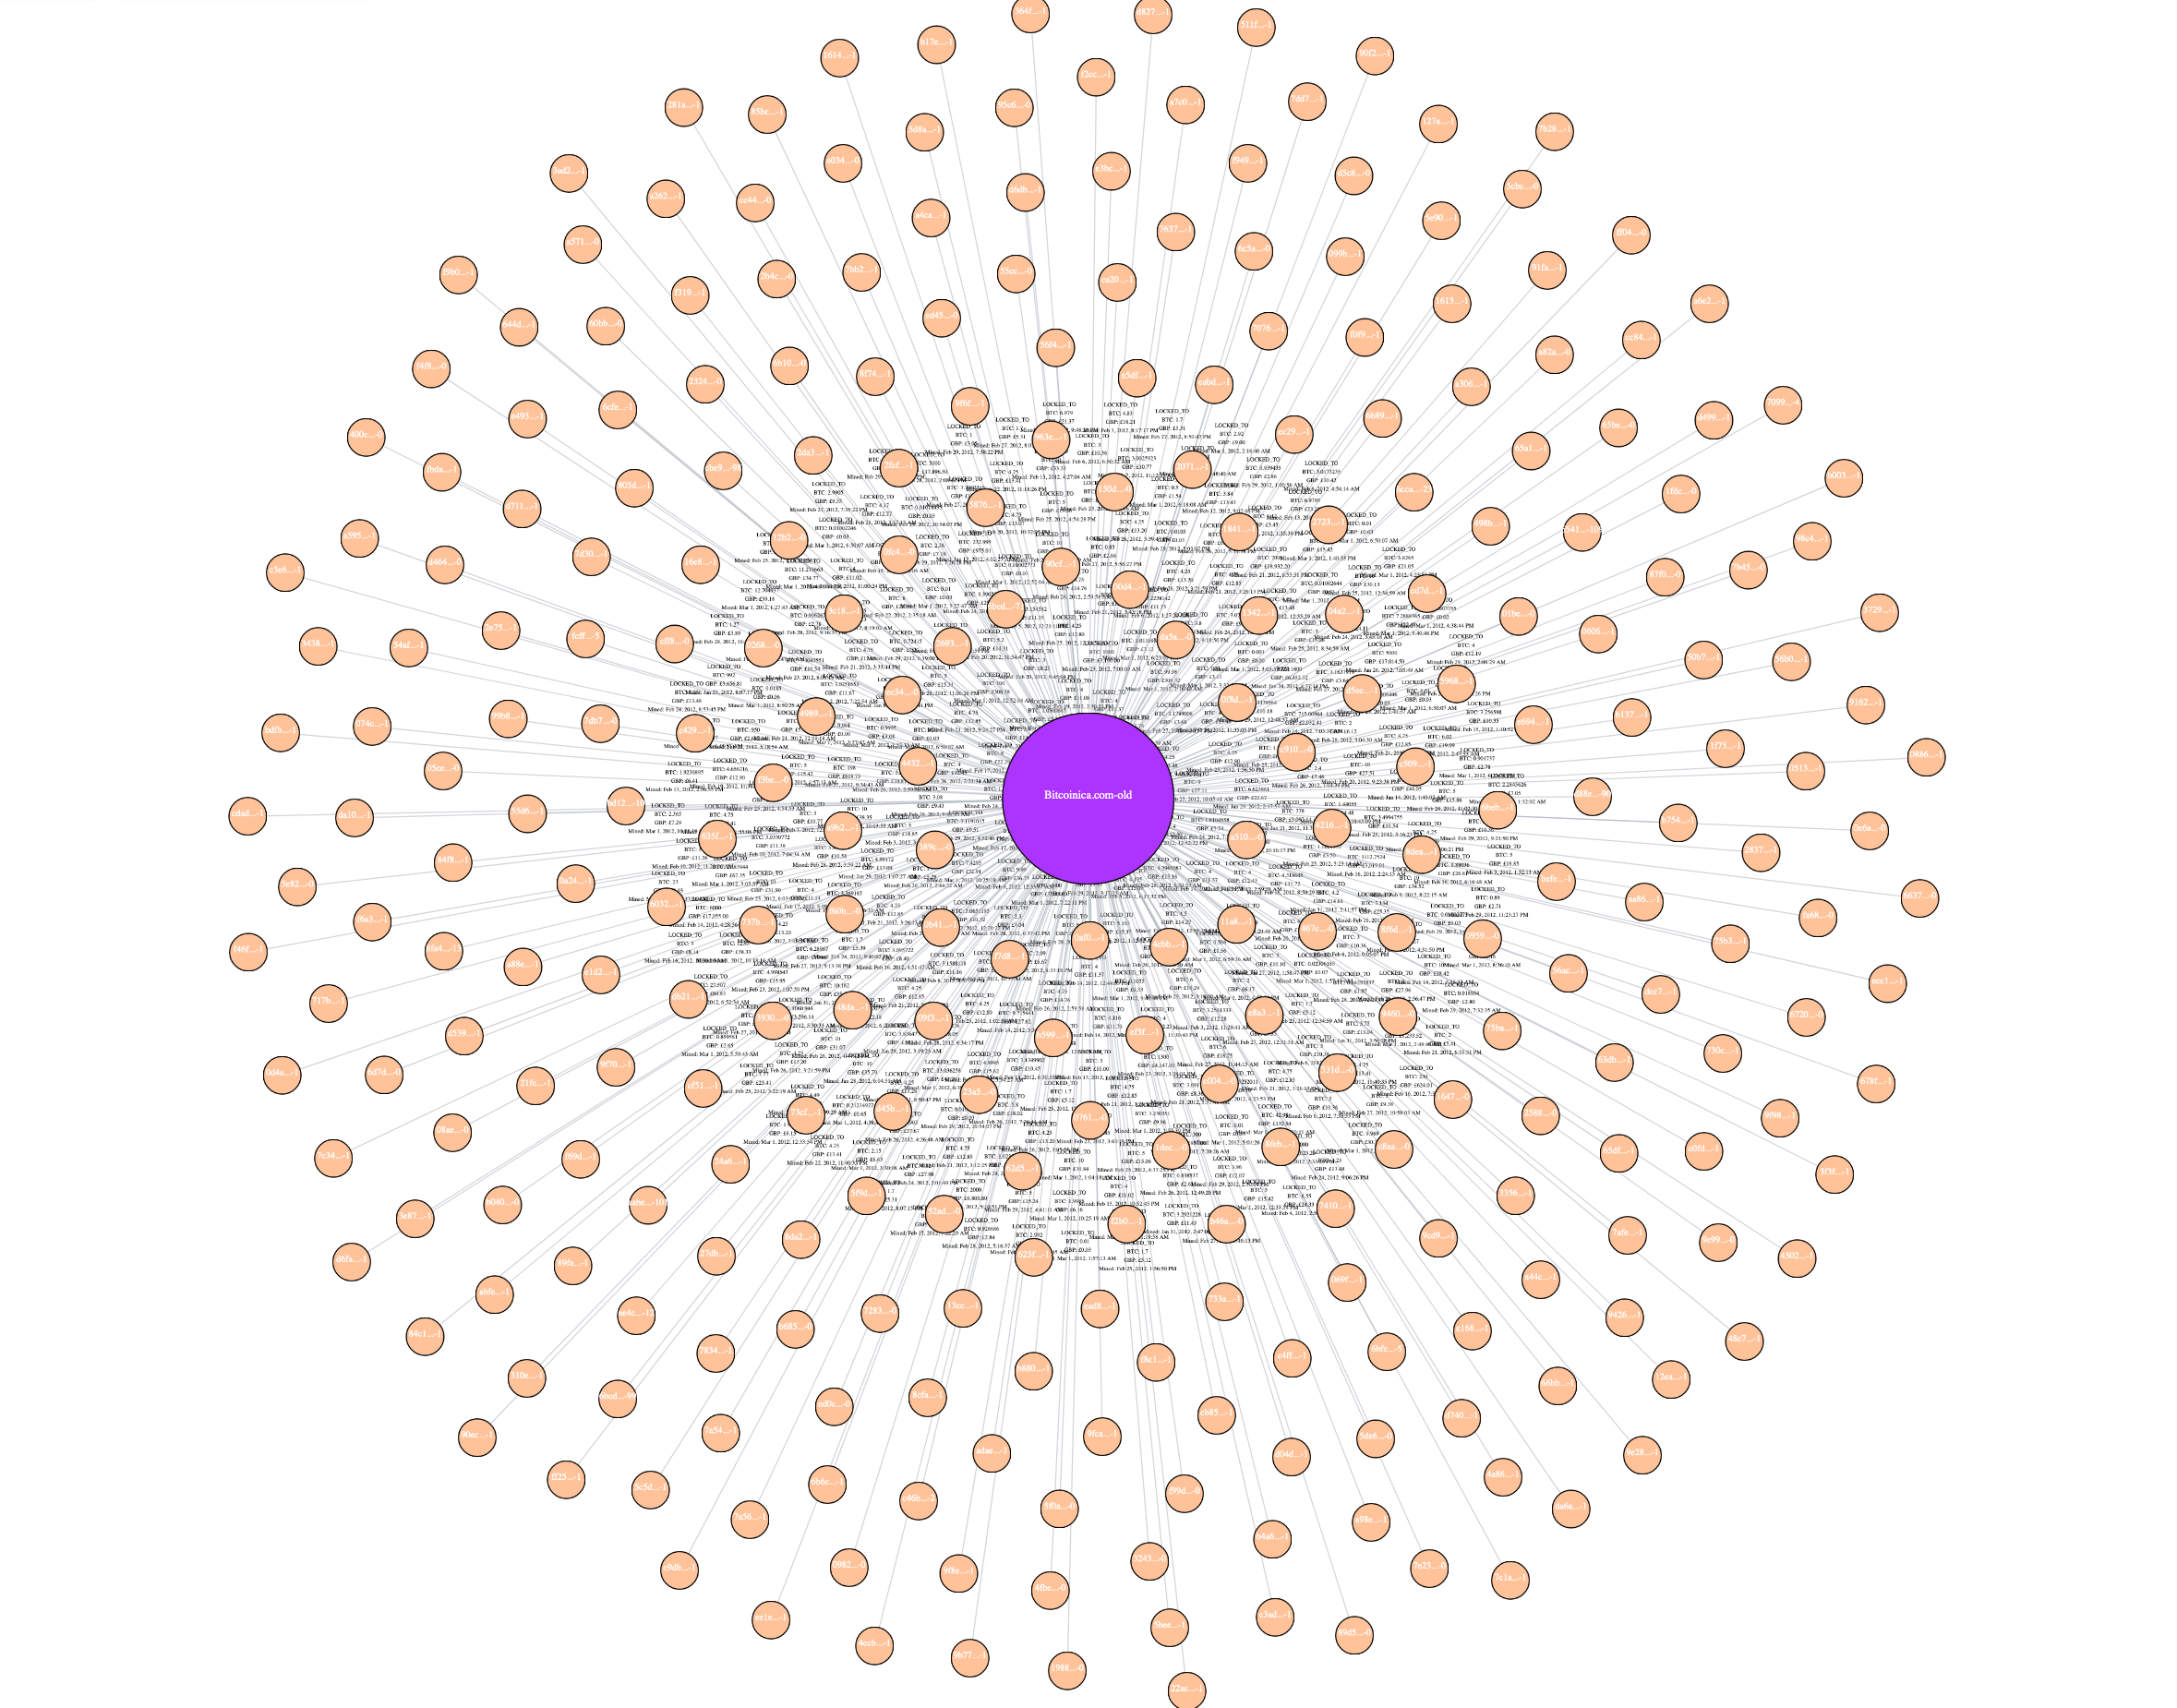
\includegraphics[width = 15cm]{./figures/theft-all-txs-1st-march}\\[0.5cm]
  \caption{A screenshot of the view when searching for entity Bitcoinica.com, filtered by date on 1st March 2012 only}.
  \label{fig:theft-no-filter}
\end{figure}

Obviously the huge amount of information shown in figure \ref{fig:theft-no-filter} is not feasible to digest and understand; therefore we navigated back to the search form to start refining the filters to help better specify what we are looking for. 
\\\\
I first added price filters in order to show only the high value transactions on the 1st of March; we filtered transactions to only show outputs that were spent of value more than $1000BTC$. 
\\\\
I then proceeded to inspect the outputs that were spent on the 1st of March that were of the greatest value [see fig \ref{fig:theft-highest-value-outputs}]. By doing so, and expanding out several other high value outputs spent on that day, we were able to identify transactions that spent a large amount of funds. We considered these transactions as suspicious.
\\\\
The suspicious transactions we identified through this process due to the size of funds they spent on this day were:
\begin{itemize}
\item \texttt{7b45c1742ca9f544cccd92d319ef8a5e19b7dcb8742990724c6a9c2f569ae732}: This transaction in total spent \textbf{20,555.1 BTC} - sending all \textbf{20,555 BTC} to one address and \textbf{0.01 BTC} to another. Using the neighbour expansion feature, we traced the bulk of the funds: 

20555BTC to 1DMuVKe9PKpx3dbs2b2MnXuVmLfA4drHif\\
25000BTC to 128u4nNS2DCbPk61aNAXLUTsHZt5FAEtit
24900BTC to 18E4d3JtQNyUBdxQ4y8ck6RUKXEb7W4KA7
23900BTRC to 1D56cDkVmoNGw7YmewL5boFwHyzEgDpygE
23399BTC to 1LJn39nzrwqM8MkevfSDCa1uVZCgJSTMtq
22399BTC to 13Fd5f8yFZCAAbtKQiNcWUmdbUNpVpznA6
21899BTC 1HZHp77ftbAEy4PQc8wuAahvPnpZHKMfmc
16899BTC 1Czhv7mDRNPMrzU9Ja7QkYSAvforGKQ2mv + 500BTC to 1Q3bsvTBcWF32Bt8FZgKAx7s43crvN9RVi (did not spend same day until July 31st 2012)
16900 to 1Q3bsvTBcWF32Bt8FZgKAx7s43crvN9RVi (spent next day on second of march)
17000 to 1BKF8kXHsNdQk6f5FognK4ZJCCBifE8ugm
15476 to 1MXe7zFRHx9KMwGKAGi2GvTbsHFDgVjcEw
12544 to 15GPUomoHVJbBsgY6eWdsKKaV3dywL5poj
12044 to 12F1GhUbVJvNW6ki1fRG1ZgeTkm2FixLLi


[9264 to 14Qr38dfmXZJUuxYaJxaTjg7yYcj5GDTqy - supernode cluster which 1BKF8kXHsNdQk6f5FognK4ZJCCBifE8ugm with earlier 17000 was paid to]

Supernodes then collect funds in tx, sends 9751 to 18ywk3t8XFtkEqMJt8hPG14D3gzTshB4YW

Does not spend funds till 4th August 2012
This seems to be the beginning of another chain, spending sums of 100-1000 BTC (usually round numbers such as 100m 200, 500 etc) in each transaction, each transaction having only two outputs until the main large funds reduce down to just over 1000BTC with transaction fbab826df674b1e2ae3bedfc566f2692b8940ac1058605fe549753b34ebd8f0d. This seems to be the end of the peeling chain, as transactions now have several inputs and smaller outputs aren't round numbers, more common to normal spending, therefore and look less characteristic of a peeling chain. 


At this point, we wished to continue the investigation by following the address 1Q3bsvTBcWF32Bt8FZgKAx7s43crvN9RVi into the next day. 

\item \texttt{0268b7285b95444808753969099f7ae43fb4193d442e3e0deebb10e2bb1764d0}


This was a sum of 10000 BTC sent to address 1AaXeH5DuP6FpPxdCn9RGXKWhSG4r9Hq9q. Not spent until March 27th 2012.


\item \texttt{a82ad85286c68f37a2feda1f5e8a4efa9db1e642b4ef53cb9fd86170169e5e68}
\item \texttt{a57132e2cbc580ac262aa3f7bac1e441d6573f9633118bc48009618585a0967e}
\item \texttt{901dbcef30a541b8b55fae8f7ad9917ef0754bda5b643705f3773e590785c4d3}
\item 

\end{itemize}

\begin{figure}[h!]
  \centering
  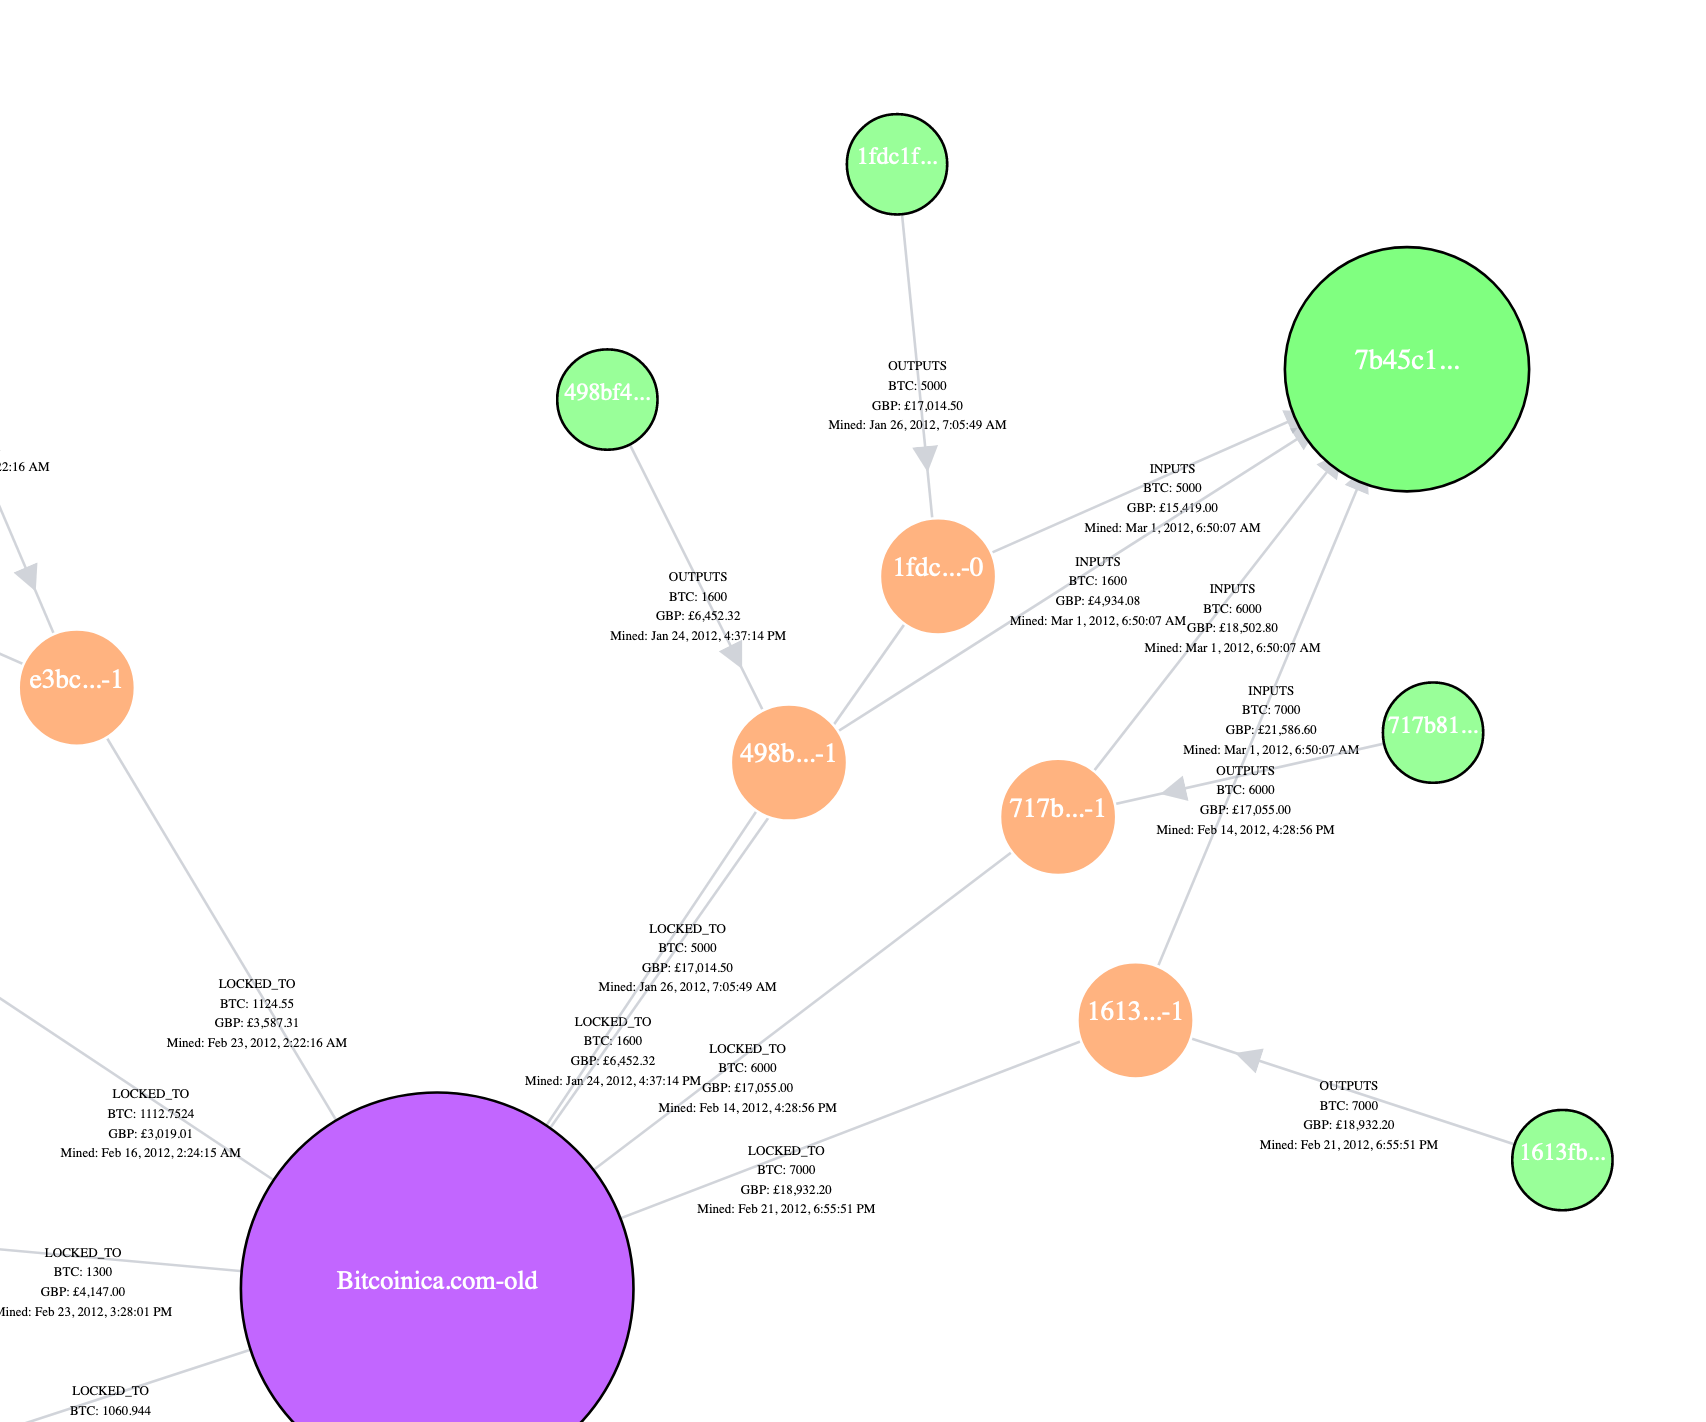
\includegraphics[width = 15cm]{./figures/theft-high-value-tx}\\[0.5cm]
  \caption{A screenshot of the view when searching for entity Bitcoinica.com, filtered by date on 1st March 2012 and by price, showing outputs spent with value > 1000BTC. Showing specifically the transaction spending the highest value outputs}.
  \label{fig:theft-highest-value-outputs}
\end{figure}

\subsection{Areas identified for improvement}
While performing the investigation using the tool, there were several features we imagined would have been useful in assisting us with the investigation, but are not currently provided by the tool. These features are:
\begin{itemize}
    \item Better distinction between incoming and outgoing funds (different colour links?), and potentially the ability to hide/show either incoming or outgoing only.
    \item Caching search parameters: Many times we would view the result of a search and need to tweak with the filtering parameters, however, the original search data is not cached and needed to be re-entered which was time-consuming.
    \item Functionality to automatically identify peeling chains and organise the layout to show the main flows. 
\end{itemize}

want order by desc/asc with price

identify outputs to which addresses in supernode
ability to check if an address belongs to a supernode 


\subsection{Missed Objectives}
\todo{complete}
Continuous updates via Kafka
Change address clustering

\todo{drawback - only up to block 570k}

only using one source for entity information 

metrics for number of clicks etrc

\todo{path finding correctness test}

multi input is now a thing - https://ieeexplore.ieee.org/abstract/document/8260674

evaluate using sarah micklejogn exampel 


\subsection{Clustering Correctness}
We can verify the correctness of clustering by immediate neighbours by searching for a transaction known to have several inputs locked to distinct addresses. For example, we were able to verify the correctness of clustering with immediate neighbours using address \texttt{17jkFTQuYaGssazzqZ6CTHgRVQYRgLmf34}. This address inputs transaction \\\texttt{8897ea9ceaf18a546cdc513b9179bae31a462ee5bf47818eb7ba909082d11777}, and also has inputs from 9 other distinct addresses. The clustering algorithm then produces a cluster of 10 addresses that are considered to be controlled by the same user. 
\\\\
I now verify the transitive clustering behaviour of the algorithm.  
To achieve this, we mutated a local Neo4J database containing a subset of the Bitcoin Blockchain (only blocks 0-2000). 
\\\\
I manually located an instance of addresses that can be clustered transitively using this heurisitc. The visual representation of the connections existing between two transitively linked addresses can be seen in figure \ref{fig:neo4j-transitive-clustering-screenshot}. The 3 addresses in this screenshot (in green) are \texttt{15oUEZFKAC8E8BTLt1s1jx4fPxumwB3ecr}, \texttt{17iqXQcGfjjHSsJK993mu75sPBnLFSEp8F} and \texttt{1Js6Nx1822qSjETsnp2kkhQFwmRNRWxgak}. They are linked through two transactions (in blue) \texttt{04dc7226529763e8c15d58171d1ac1e28cb6b8d3165005765e65757c7b219d2d} and \texttt{c7a4bb767027a4382462c32b6a824a53e2715d833c0d86e9676a4fbddedca0a9}. 
\\\\
I was able to verify that executing the clustering algorithm included all 3 of these addresses in the result, and became confident of the correct transitive behaviour of the implementation of the clustering algorithm. 

\begin{figure}[h!]
  \centering
  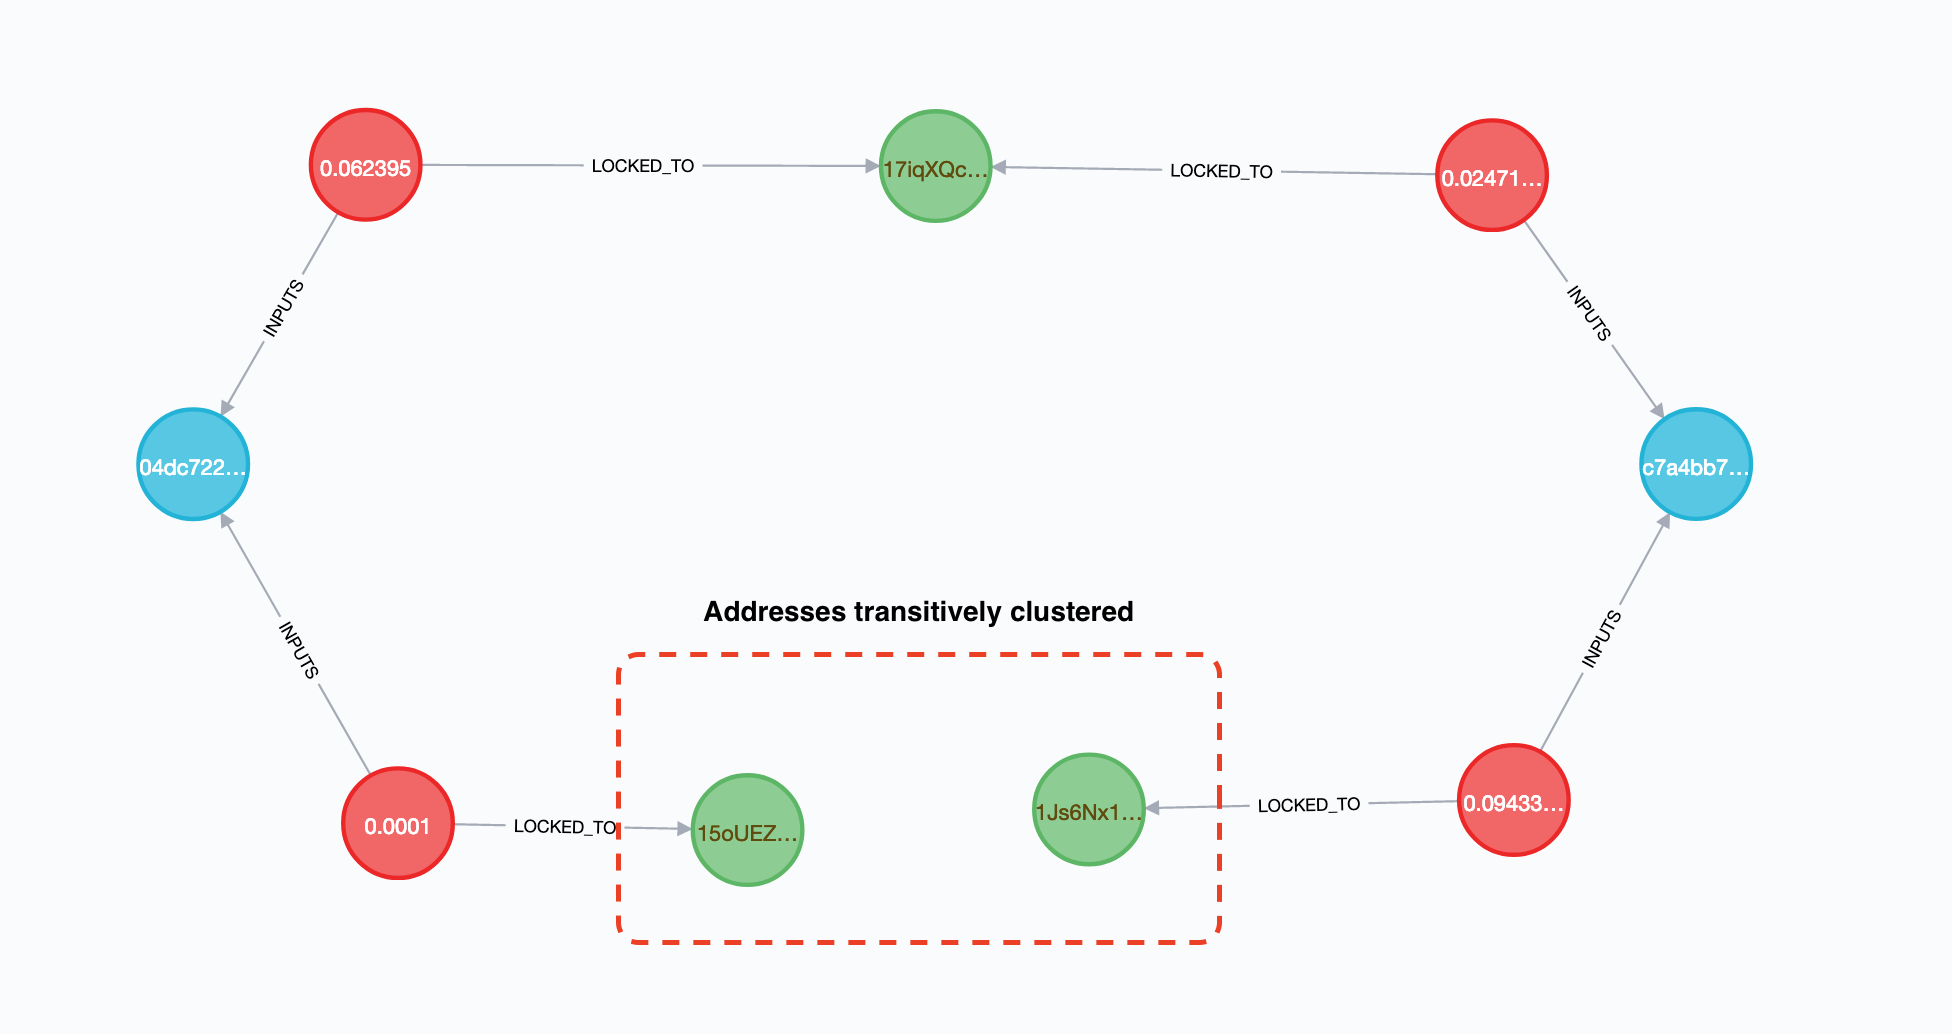
\includegraphics[width = 15cm]{./figures/neo4j-screenshots/addresses-transitively-clustered}\\[0.5cm] 
  \caption{A screenshot of the Neo4J UI : Visual representation of addresses that are clustered transitively.}
  \label{fig:neo4j-transitive-clustering-screenshot}
\end{figure}

\section{Comparisons with existing tools}
As described in the background section \ref{background-existing-tools}, there currently exist some tools, both free and proprietary, that could be used to help carry out a digital forensic investigation. In this section, we compare the tool developed in this project both qualitatively and quantitatively.

\subsection{Wallet Explorer}
Given the example above, where we would like to investigate a theft that occurred from Bitcoinica.com, we would need to take the following steps on the Wallet Explorer site:
\begin{itemize}
    \item Navigate to walletexplorer.com \textbf{one click}
    \item Click bitcoinica.com old \textbf{one click}
    \item Scan the transactions date table for a date matching 1st March 2012 (the theft date): this required using the table pagination controls until transactions for March 1st 2012 shows : \textbf{one click}
    \item We now search for the large transaction values and see a outgoing transaction of 20,555 BTC and inspect that transaction \textbf{one click}. TXID is \\\texttt{    7b45c1742ca9f544cccd92d319ef8a5e19b7dcb8742990724c6a9c2f569ae732}
    \item We see the output address of transaction is \texttt{ 1DMuVKe9PKpx3dbs2b2MnXuVmLfA4drHif} \textbf{one click}
    \item Can click on 'next tx' to follow the flow of funds: pays the funds to address \\\texttt{128u4nNS2DCbPk61aNAXLUTsHZt5FAEtit}
    \item Can follow the peeling chain in same manner as before with one click on 'next tx' - \textbf{n clicks for n steps of the peeling chain}
\end{itemize}

In comparison, the steps taken to obtain similar data using \textit{Radar} developed in this project are:
\begin{itemize}
    \item Navigate to \textit{Radar}: \textbf{one click}
    \item \textbf{One click} to initiate the search for the 'Bitcoinica.com' wallet with all date and price filter applies such that only nodes for 1st March are shown and only transactions of high BTC value are shown 
    \item Can instantly identify the high value transaction \\\texttt{7b45c1742ca9f544cccd92d319ef8a5e19b7dcb8742990724c6a9c2f569ae732} so can trace the funds from that output by double-clicking and seeing the address \\\texttt{128u4nNS2DCbPk61aNAXLUTsHZt5FAEtit} : \textbf{one click}
    \item Can now follow the peeling chain for one click for each step \textbf{n clicks for n steps of the peeling chain}
\end{itemize}
We use a quantitative measure of the 'number of user clicks' to measure the number of steps that need to be taken to follow a peeling chain after a theft for a given wallet. 
\\\\\
Using Wallet Explorer, we find we require \textbf{5 + n clicks} whereas using \textit{Radar}, just \textbf{3 + n clicks} when following \textbf{n} steps of a peeling chain from the same theft.
\\\\
Qualitatively, \textit{Radar} made following the peeling chain far easier as you are given the option to see where funds peel off to from any stage - using walletexplorer, you can only see one step of the peeling chain at any one time; \textit{Radar} shows the entire path and overall paints a better picture of the flow of funds. 
\\\\
Additionally, a factor not considered in the above click metric is if the user wanted to know what the value of each stage was in its respective fiat currency. \textit{Radar} integrates the converted values into the UI; using Wallet Explorer, we would have to add several more clicks to measure the effort required to convert the transaction values to a fiat currency.

\subsection{Blockchain Explorer}
We compare the functionality of \textit{Radar} to that provided by Blockchain Explorer [see \ref{background:blockchain-explorer}]; we do not use the clicks metrics as before due to variations in the functionality provided by each tool. Therefore, we carry out a qualitative comparison.
\\\\
Blockchain explorer does not provide the functionality to search by an entity name such as 'Bitcoinica.com'; therefore, we would struggle to identify the transactions related to a theft from this entity. 
\\\\
Skipping the step of identifying suspicious transactions and presuming we had a particular transaction of interest, such \texttt{7b45c1742ca9f544cccd92d319ef8a5e19b7dcb8742990724c6a9c2f569ae732}. At this point, we have similar functionality as provided by Wallet Explorer and can follow links to see each transaction in isolation and trace the peeling chain, but with the same drawbacks in comparison to \textit{Radar} that it does not show the whole path. 
\\\\
A feature that Blockchain Explorer does provide is a conversion into USD; however, this is not a historical conversion, this is a conversion according to the current exchange rate. For instance, when viewing the above transaction on the site on 12th June 2019, we see it shows the 20,555 BTC output sent to address \texttt{DMuVKe9PKpx3dbs2b2MnXuVmLfA4drHif} has a value in USD of \$164,885,221.3. However, when this theft occurred, bitcoin had a value that was magnitudes lower than its value today, therefore this conversion on Blockchain Explorer may not be very useful to understanding the value of transactions that occurred during the 2012 theft. 

\subsection{Blockpath}
We compare the functionality offered by Blockpath [see \ref{background:blockpath}] to \textit{Radar}. Again, we do not use the clicks metric as before due to vast variations in the functionality offered. Therefore, we carry out a qualitative comparison only,
\\\\
Similar to Blockchain Explorer, Blockpath provides the ability to search for particular transactions and addresses, but not the ability to find all activity for an entity such as 'Bitcoinica.com', so it would be difficult to use this tool to identify a suspicious address. 
\\\\
A distinguishing feature Blockpath provides that the other tools do not is a graphical interface. Using a given suspicious transaction ID \\\texttt{7b45c1742ca9f544cccd92d319ef8a5e19b7dcb8742990724c6a9c2f569ae732}, we attempt to follow the peeling chain using the graphical interface. Similar to \textit{Radar}, funds can be followed by double clicking on nodes which will expand the next step in the flow of funds. 
\\\\
A feature of Blockpath's graph visualisation which we believe is very useful is the timeline on the left-hand side [see fig \ref{fig:blockpath-graph-ui-time-organisation}], and organisation of nodes vertically based on their timestamps. The organisation of nodes in Blockpath's graph visualisation is, therefore, more meaningful than in \textit{Radar}, where the arrangement is random. 
\\\\
However, Blockpath does not provide the option to filter such that only transactions for a particular date or value are shown; this, therefore, leads to bloat of the graph which could make tracing the flow of funds more difficult [see figure \ref{fig:blockpath-graph-ui}]. 

\begin{figure}[h!]
  \centering
  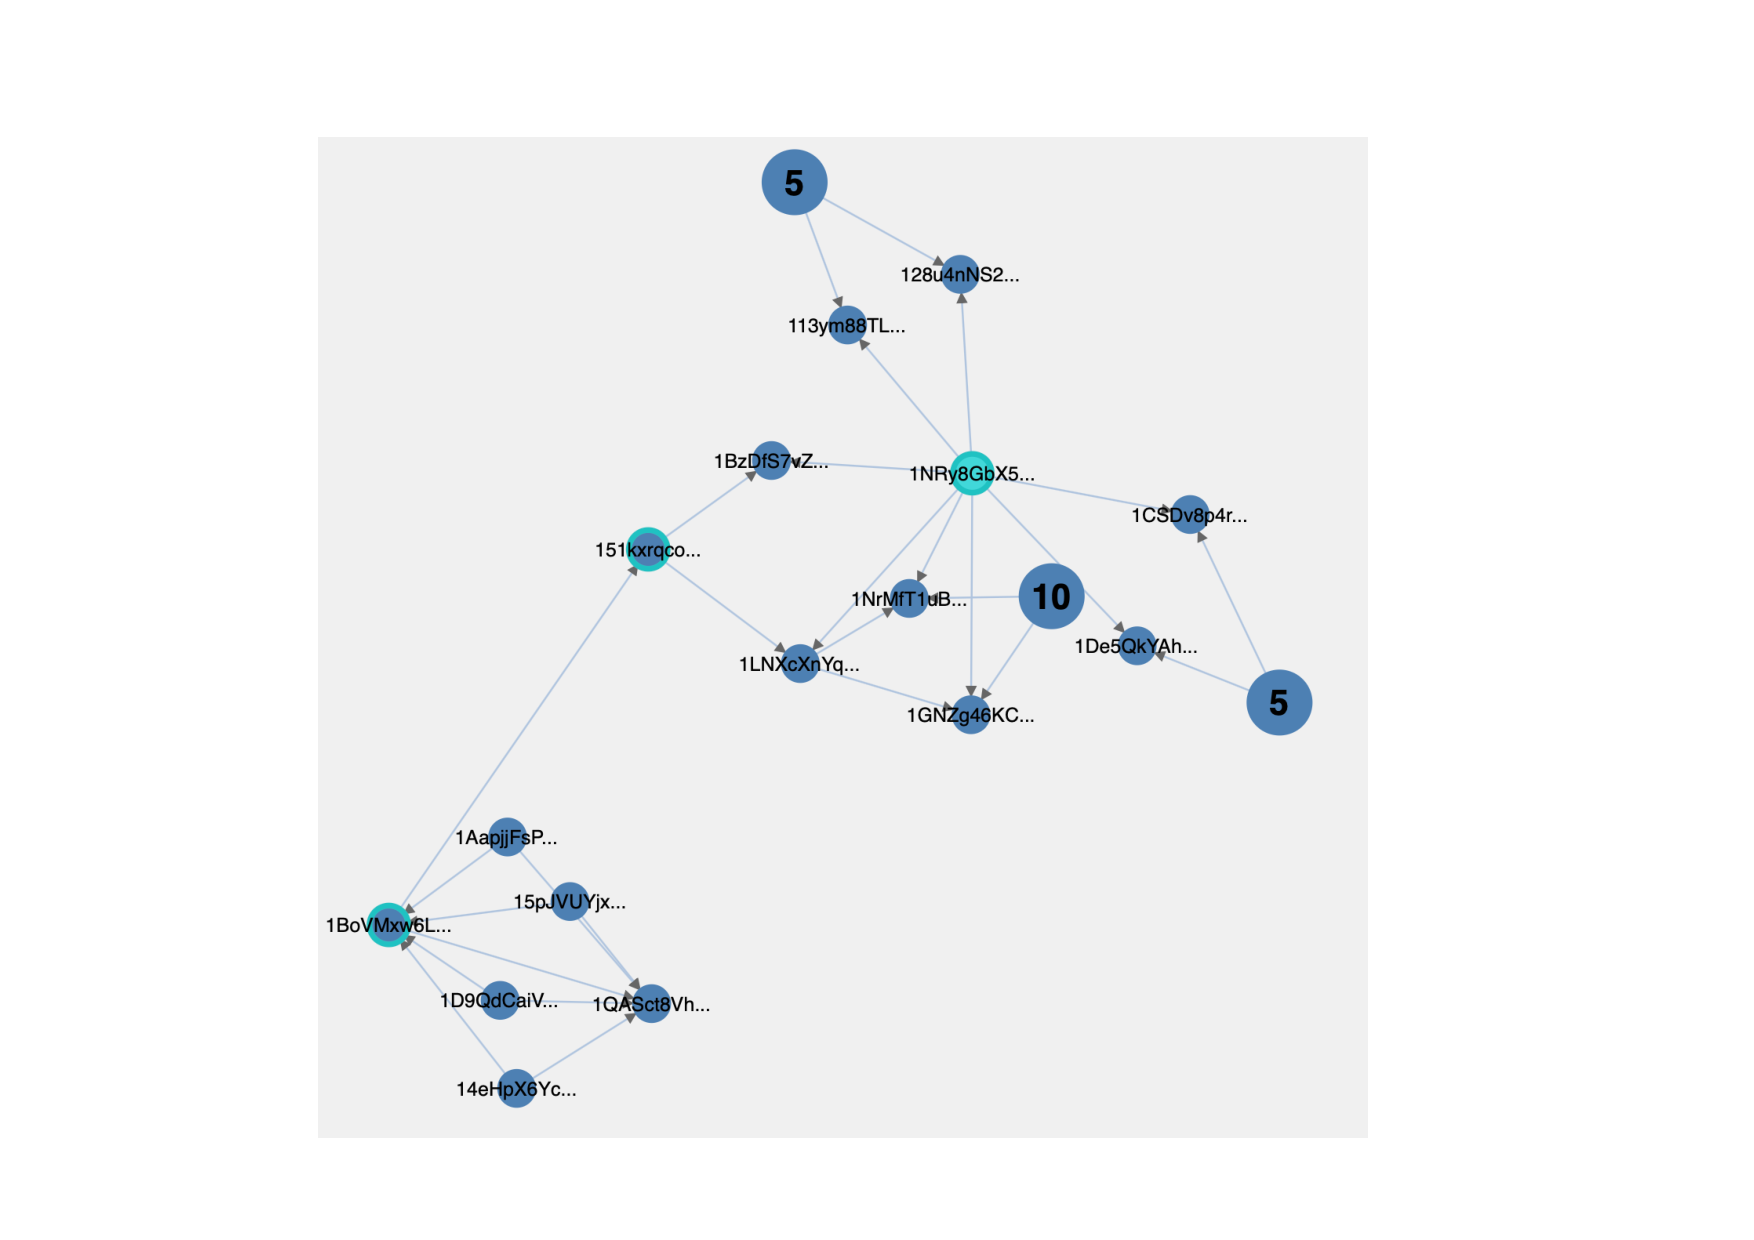
\includegraphics[width = 15cm]{./figures/blockpath-evaluation}\\[0.5cm] 
  \caption{A screenshot of the Blockpath graphical interface feature.}
  \label{fig:blockpath-graph-ui}
\end{figure}

\begin{figure}[h!]
  \centering
  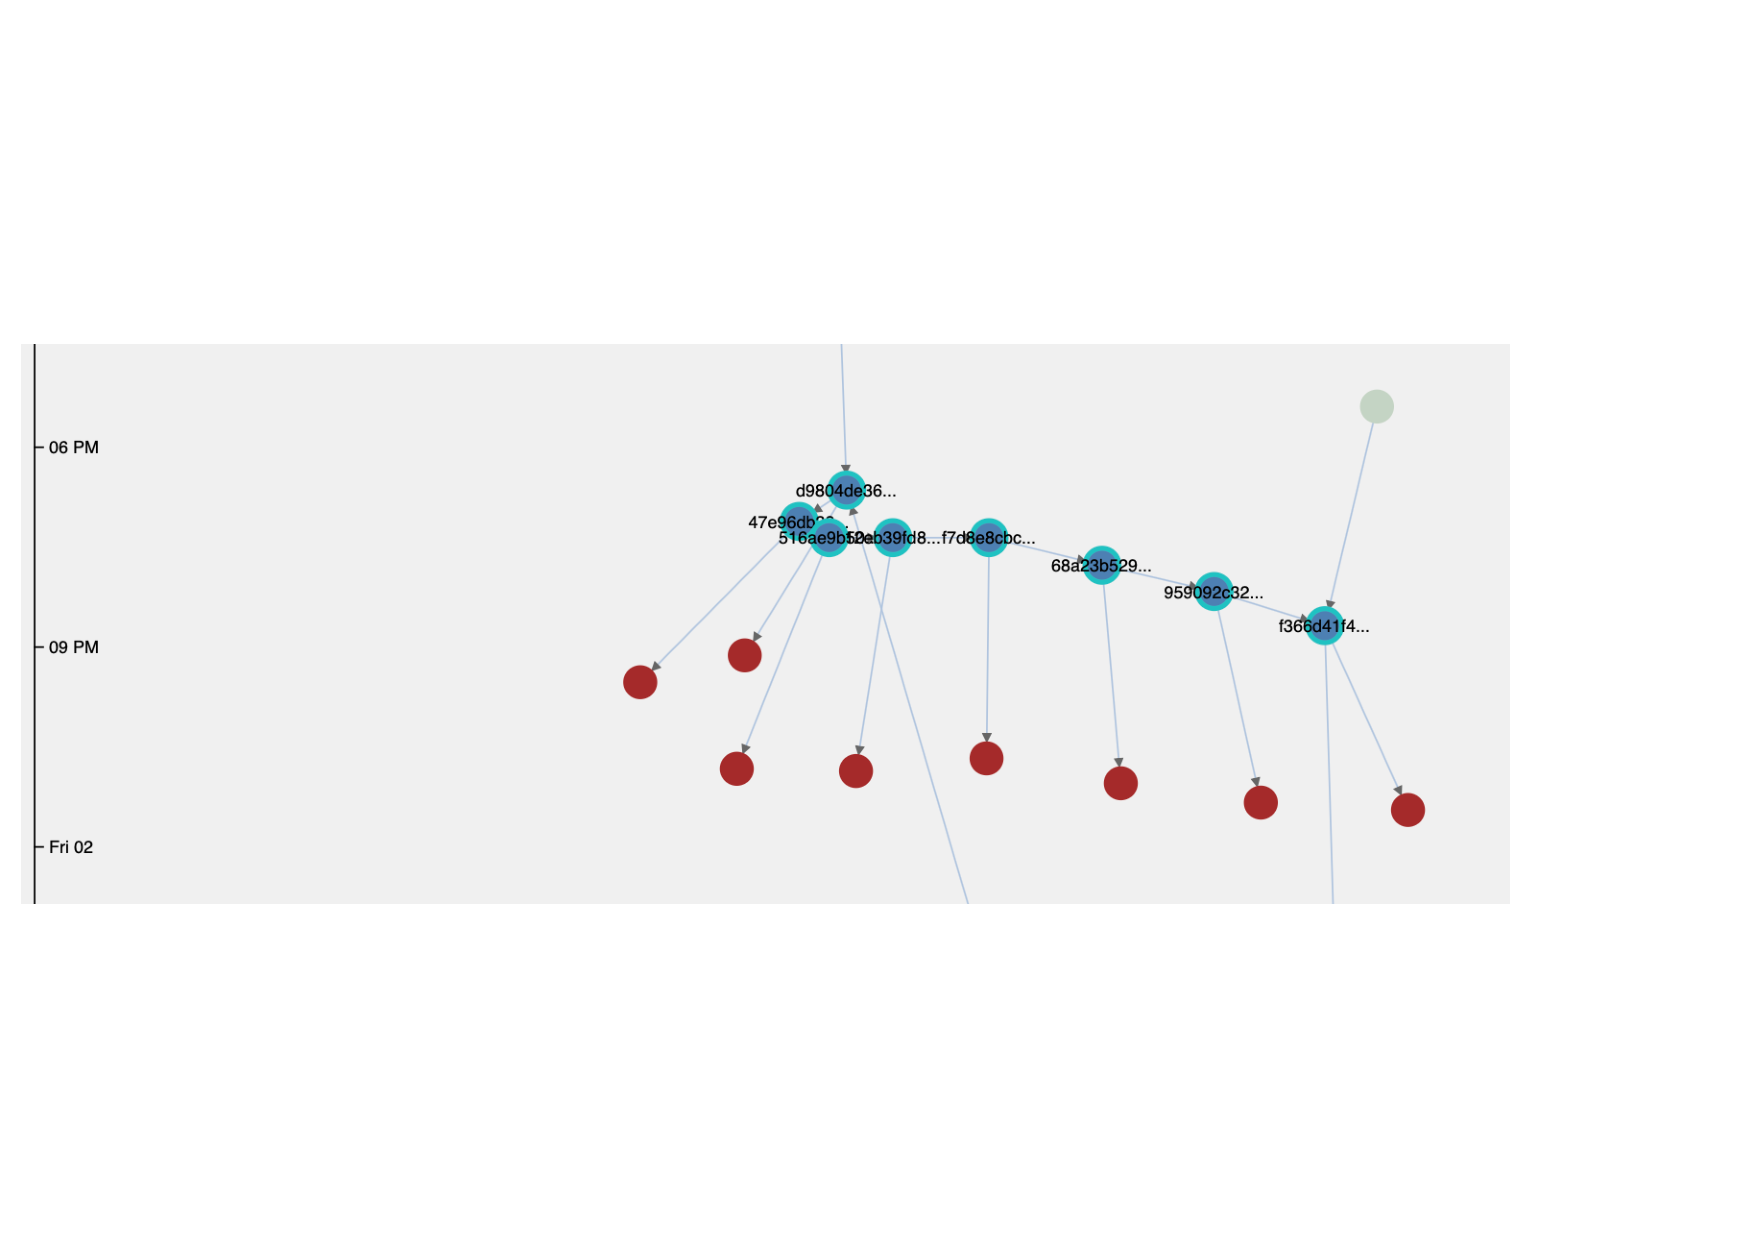
\includegraphics[width = 15cm]{./figures/blockpath-time-org}\\[0.5cm] 
  \caption{A screenshot of the Blockpath graphical interface feature, also showing timeline.}
  \label{fig:blockpath-graph-ui-time-organisation}
\end{figure}